\documentclass[tikz, margin=3mm, 12pt]{standalone}
\usetikzlibrary{shadows}

\usepackage[T1]{fontenc}		% Selecao de codigos de fonte.
\usepackage[utf8]{inputenc}		% Codificacao do documento (conversão automática dos acentos)


\definecolor{silver}{HTML}{D6D6D6}
\usepackage{fontawesome, booktabs,  tabularx, multirow}
\usepackage{colortbl}


\newcommand{\thehspace}{5.8cm}

\newcommand{\sethspace}[1]{
	\renewcommand*{\thehspace}{#1}
}
\renewcommand{\arraystretch}{1.5}


\newcommand{\disciplina}[5]{
	
	 \begin{tabularx}{\linewidth}{r  | X  }

        \multirow{3}{*}{\rotatebox[origin=c]{90}{\small\texttt #1}} &  {\large\bfseries \MakeUppercase{#2} \hfill (#5)}   \\ 
                \cline{2-2}
        & {\large\texttt{#3} }  \\
        \cline{2-2}
        & \large\texttt{#4}   \\        
    \end{tabularx}
      
}

\newcommand{\disciplinalivre}[4]{
	 \begin{tabularx}{\linewidth}{r  | X  }
        \multirow{2}{*}{\rotatebox[origin=c]{90}{\small\texttt #1}} & {\large\bfseries \MakeUppercase{#2} \hfill (#4)}   \\ 
                \cline{2-2}      
        & \large\texttt{#3}   \\     
        \end{tabularx} 
}



\begin{document}

	\newcommand{\paramsforfirst}{node distance=5cm, text width=8cm}


    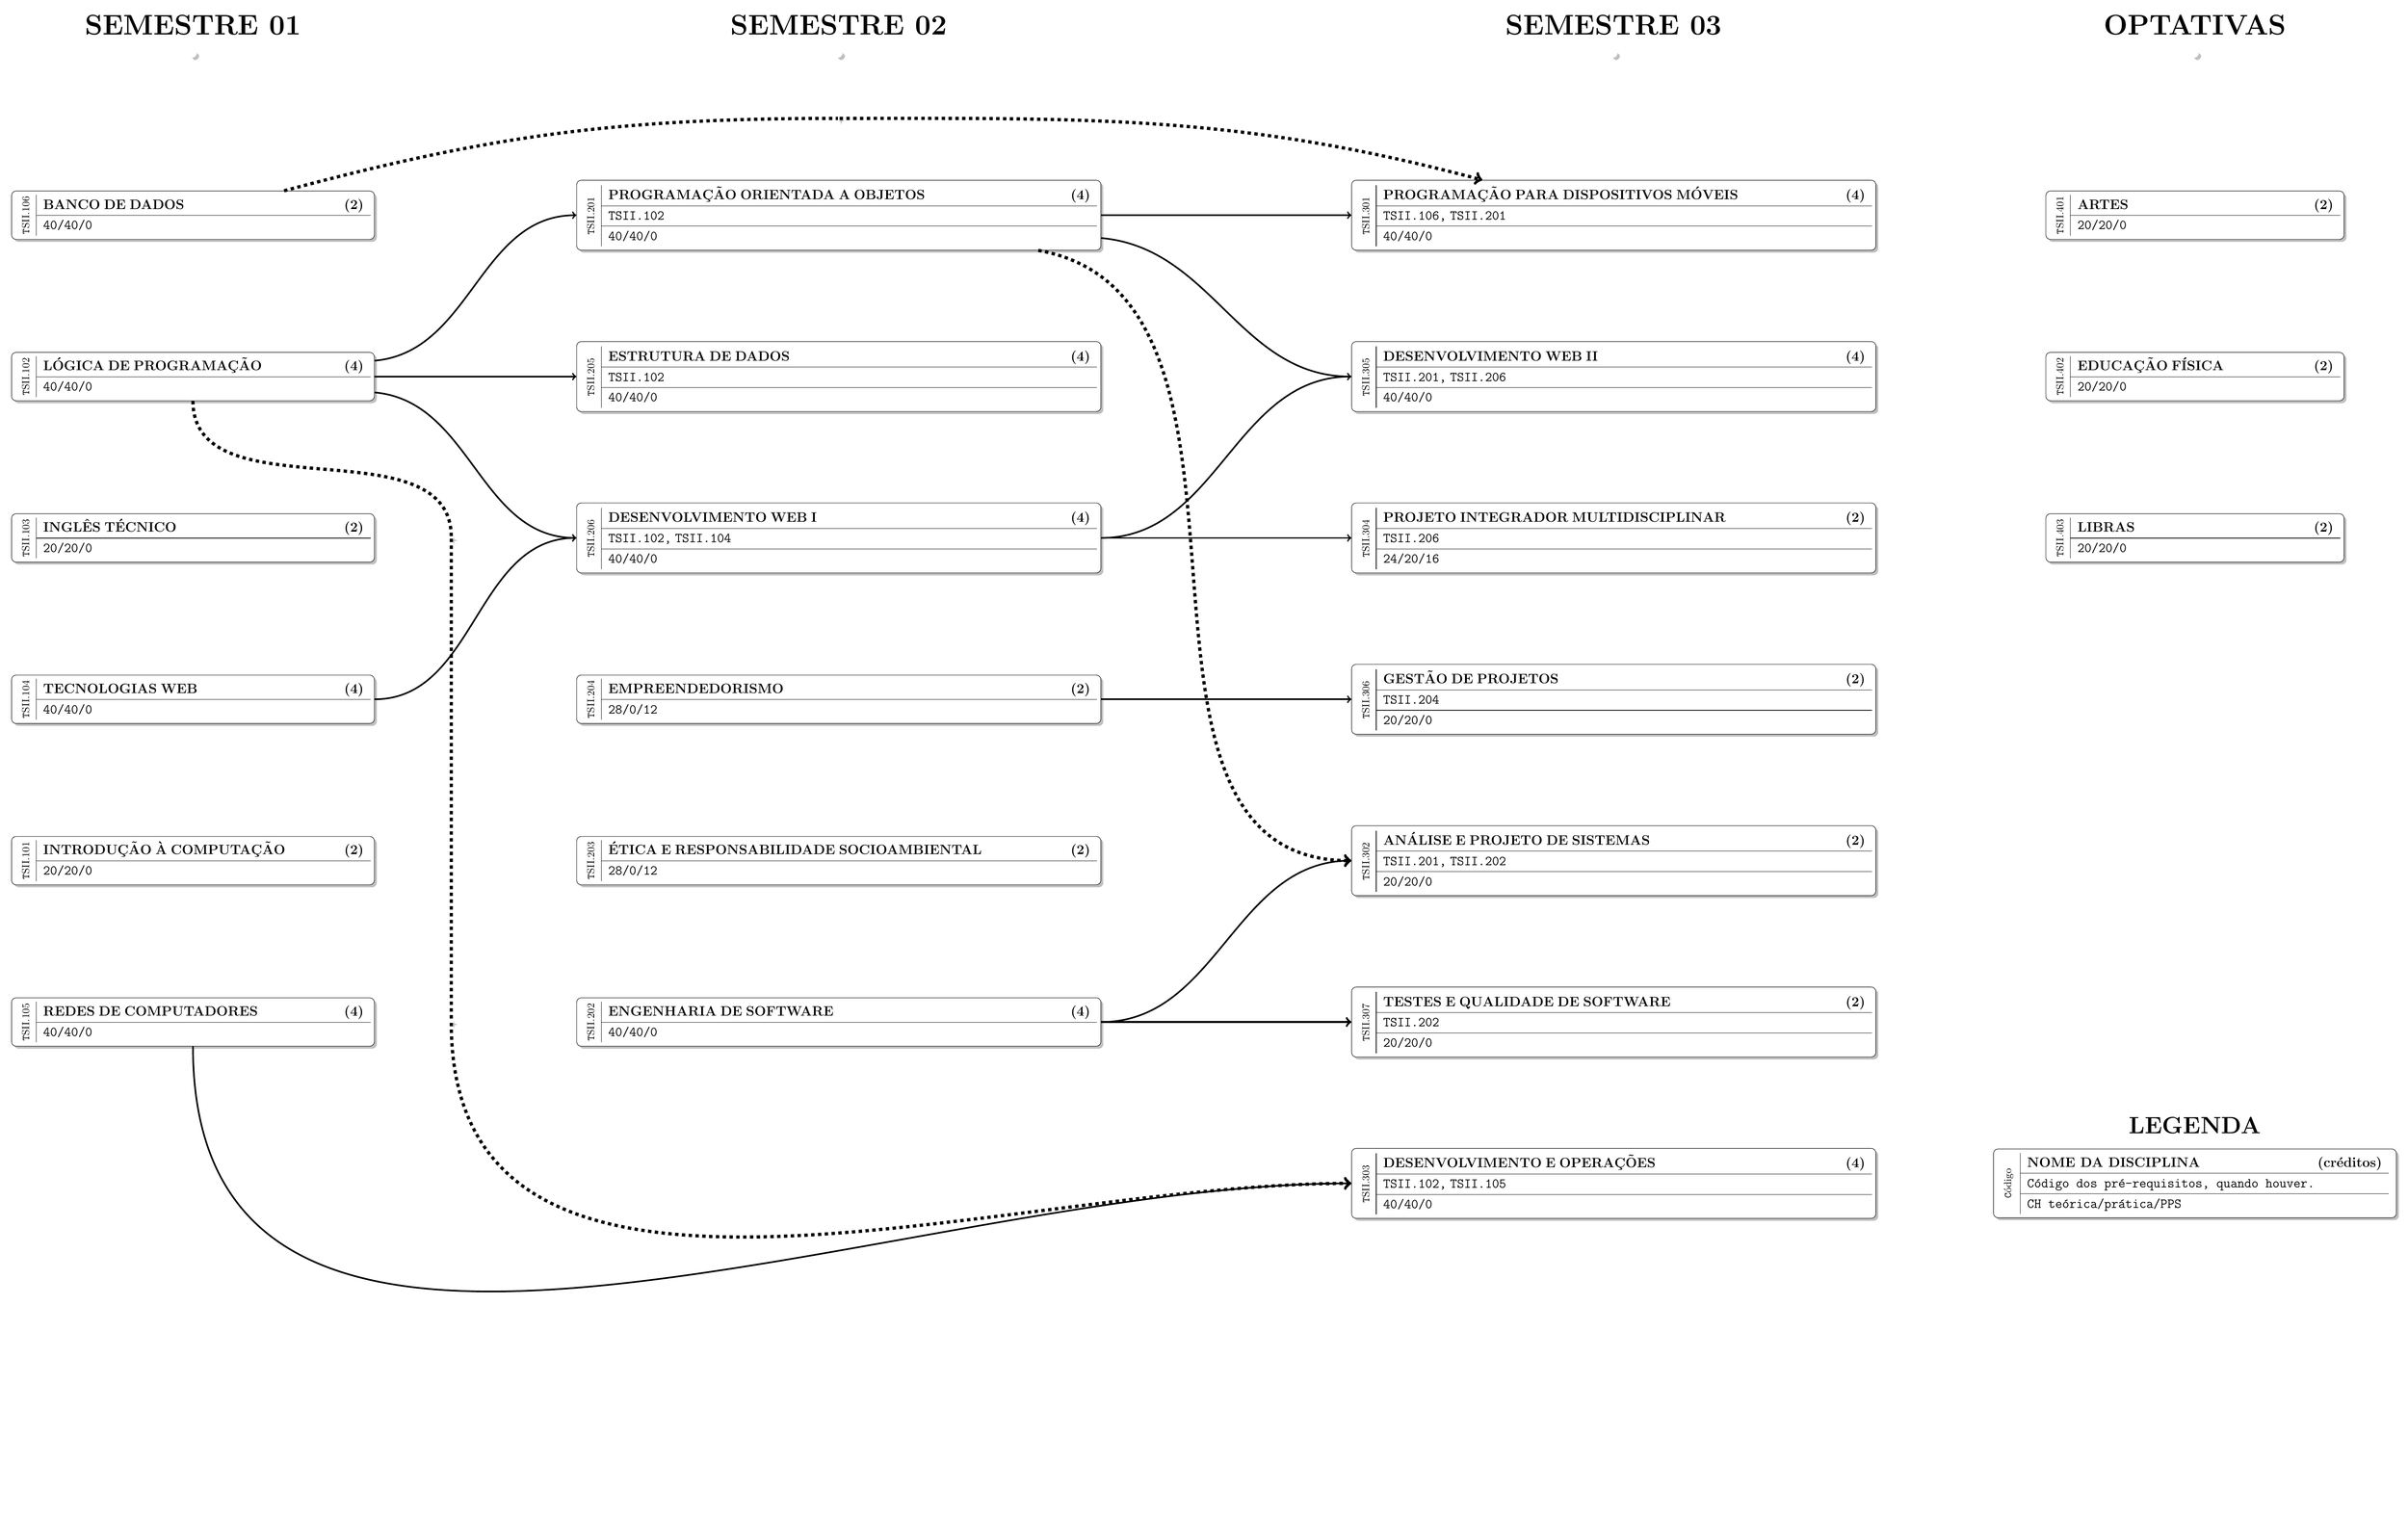
\begin{tikzpicture}[ every node/.style = {draw, fill=white, drop shadow, rounded corners}, every label/.append style = {
     label distance=1em, font=\scriptsize,  every shadow/.style={opacity=0}}]
     
     \sethspace{6cm}
     
     
     %%% TOPO
     \node [draw=none, label={\Huge\textbf{SEMESTRE 01}}]  (S1) {};

     \node [draw=none, label={\Huge\textbf{SEMESTRE 02}}, right of = S1,  node distance=20cm]  (S2) {};
     
     \node [draw=none, label={\Huge\textbf{SEMESTRE 03}},, right of = S2,  node distance=24cm]  (S3) {};     

     \node [draw=none, label={\Huge\textbf{OPTATIVAS}},,  right of = S3,  node distance=18cm ]  (OPT) {};     
     
     %%% MIOLO
     
     
     %% RODAPÉ

	
	% S01
	\node [,below of= S1, node distance=5cm, text width = 11cm]  (BD) {
		\disciplinalivre{TSII.106}{Banco de Dados}{40/40/0}{2}
	};
	\node [,below of= BD, node distance=5cm, text width = 11cm]  (LOGICA) {
		\disciplinalivre{TSII.102}{Lógica de programação}{40/40/0}{4}
	};
	\node [,below of= LOGICA, node distance=5cm, text width = 11cm]  (INGLES) {
		\disciplinalivre{TSII.103}{Inglês Técnico}{20/20/0}{2}
	};
	\node [,below of= INGLES, node distance=5cm, text width = 11cm]  (WEBD) {
		\disciplinalivre{TSII.104}{Tecnologias WEB}{40/40/0}{4}
	};
	\node [,below of= WEBD, node distance=5cm, text width = 11cm]  (INTRO) {
		\disciplinalivre{TSII.101}{Introdução à Computação}{20/20/0}{2}
	};
	\node [,below of= INTRO, node distance=5cm, text width = 11cm]  (REDES) {
		\disciplinalivre{TSII.105}{Redes de Computadores}{40/40/0}{4}
	};
	
	
	
	
	% S02
	\node [,below of= S2, node distance=5cm, text width = 16cm]  (POO) {
		\disciplina{TSII.201}{Programação orientada   a objetos}{TSII.102}{40/40/0}{4}
	};
	\node [,below of= POO, node distance=5cm, text width = 16cm]  (ED) {
		\disciplina{TSII.205}{Estrutura de dados}{TSII.102}{40/40/0}{4}
	};
	\node [,below of= ED, node distance=5cm, text width = 16cm]  (DEVI) {
		\disciplina{TSII.206}{Desenvolvimento WEB I}{TSII.102, TSII.104}{40/40/0}{4}
	};
	\node [,below of= DEVI, node distance=5cm, text width = 16cm]  (EMP) {
		\disciplinalivre{TSII.204}{Empreendedorismo}{28/0/12}{2}
	};
	\node [,below of= EMP, node distance=5cm, text width = 16cm]  (ETICA) {
		\disciplinalivre{TSII.203}{Ética e Responsabilidade  Socioambiental}{28/0/12}{2}
	};
	\node [,below of= ETICA, node distance=5cm, text width = 16cm]  (ES) {
		\disciplinalivre{TSII.202}{Engenharia de Software}{40/40/0}{4}
	};
	

	% S03
	\node [,below of= S3, node distance=5cm, text width = 16cm]  (MOBILE) {
		\disciplina{TSII.301}{Programação para  Dispositivos Móveis}{TSII.106, TSII.201}{40/40/0}{4}
	};
	\node [,below of= MOBILE, node distance=5cm, text width = 16cm]  (DEVII) {
		\disciplina{TSII.305}{Desenvolvimento WEB II}{TSII.201, TSII.206}{40/40/0}{4}
	};
	\node [,below of= DEVII, node distance=5cm, text width = 16cm]  (PIM) {
		\disciplina{TSII.304}{Projeto Integrador  Multidisciplinar}{TSII.206}{24/20/16}{2}
	};
	\node [,below of= PIM, node distance=5cm, text width = 16cm]  (GP) {
		\disciplina{TSII.306}{Gestão de Projetos}{TSII.204}{20/20/0}{2}
	};
	\node [,below of= GP, node distance=5cm, text width = 16cm]  (APS) {
		\disciplina{TSII.302}{Análise e Projeto  de Sistemas}{TSII.201, TSII.202}{20/20/0}{2}
	};
	\node [,below of= APS, node distance=5cm, text width = 16cm]  (TESTES) {
		\disciplina{TSII.307}{Testes e Qualidade  de Software}{TSII.202}{20/20/0}{2}
	};
	\node [,below of= TESTES, node distance=5cm, text width = 16cm]  (DEVOPS) {
		\disciplina{TSII.303}{Desenvolvimento e  Operações}{TSII.102, TSII.105}{40/40/0}{4}
	};
	
	
	
	% OPT
	
	\node [,below of= OPT, node distance=5cm, text width = 9cm]  (ARTE) {
		\disciplinalivre{TSII.401}{Artes}{20/20/0}{2}
	};
	\node [,below of= ARTE, node distance=5cm, text width = 9cm]  (EF) {
		\disciplinalivre{TSII.402}{Educação física}{20/20/0}{2}
	};
	\node [,below of= EF, node distance=5cm, text width = 9cm]  (LIBRAS) {
		\disciplinalivre{TSII.403}{Libras}{20/20/0}{2}
	};
		
	
	%CONEXOES
	
	\draw[->, line width=0.05cm] (LOGICA) to[out=5, in=180] (POO);
	\draw[->, line width=0.05cm] (LOGICA) -- (ED);
	\draw[->, line width=0.05cm] (LOGICA) to[out=355, in=180] (DEVI);
	\draw[->, line width=0.05cm] (WEBD) to[out=360, in=180] (DEVI);
	
	

	\draw[->, line width=0.05cm] (POO) -- (MOBILE);
	\draw[->, line width=0.05cm] (POO) to[out=355, in=180]  (DEVII);
	\draw[->, line width=0.1cm,dashed] (POO) to[out=350, in=180]  (APS);	
	\draw[->, line width=0.05cm] (DEVI) to[out=360, in=180]  (DEVII);
	\draw[->, line width=0.05cm] (DEVI) -- (PIM);


	\draw[->, line width=0.05cm] (EMP) -- (GP);
	\draw[->, line width=0.05cm] (ES) to[out=360, in=180] (APS);
	\draw[->, line width=0.07cm] (ES) -- (TESTES);
	
	
	% nos inviveis
	\node [right of= INGLES, node distance=8cm, draw=none, inner sep = 0pt ] (INVTEC) {};
	\node [right of= REDES, node distance=8cm, draw=none, inner sep = 0pt] (INVTEC2) {};
	
	\draw[->, line width=.1cm, dashed] (LOGICA) to[out=270, in=90]  (INVTEC) -- (INVTEC2) to[out=270, in=180] (DEVOPS); % add no invisivel
	\draw[->, line width=0.05cm,] (REDES) to[out=270, in=180] (DEVOPS);
	
	\node [above of= POO, node distance=3cm, draw=none, inner sep = 0pt] (INVTEC3) {};
	\draw[->, line width=.1cm, dashed] (BD) to[out=15, in=180] (INVTEC3) to[out=360, in=165] (MOBILE);
	
	% LEGENDA
	\node[, label={\huge\textbf{LEGENDA}},  below of= LIBRAS , node distance=20cm,] (kkkk)  {				
		\disciplina{Código}{Nome da Disciplina}{Código dos pré-requisitos, quando houver.}{CH teórica/prática/PPS}{créditos}
	};
    \end{tikzpicture}
\end{document}